\pagebreak

\hypertarget{kuvaus-tyuxf6mallista}{%
\chapter{Kuvaus työmallista}\label{kuvaus-tyuxf6mallista}}

Tämän työn kuluessa syntyi työmalli, jota kutsun \emph{notkeaksi
tietomallin paranteluksi}. Työmalli on parhaimmillaan tilanteissa,
joissa ohjelmiston sovellusaluemalli sisältää monimutkaisia ja vain
erityisalan asiantuntijalle aukeavia käsitteitä ja käsitesuhteita.
Eduksi on myös, mikäli sovelluksen tekninen vaativuus ei ole kovin
poikkeuksellinen. Tyypillinen bisnessovellus, jossa painopiste on
sovellusalueessa, on hyvä kohde tälle työmallille.

Tämän työmallin pääperiaate on, että \textbf{sanat, kaaviot ja koodi}
ovat kolme kommunikaation muotoa, jotka täydentävät toisiaan. Kuvaan
seuraavassa tämän työmallin keskeiset ominaispiirteet.

\hypertarget{lyhyet-iteraatiot}{%
\subsubsection{Lyhyet iteraatiot}\label{lyhyet-iteraatiot}}

Lyhyet iteraatiot, joiden välissä pidetään suunnittelutapaaminen, ovat
ehdoton edellytys tietomallin ripeälle kehittämiselle. On tärkeää, että
iteraation kuluessa syntyy käyttökelpoinen ohjelmistoversio, jonka
avulla mallin toimivuutta voidaan testata ja todentaa.

\hypertarget{keskusteleva-suhde-tuoteomistajan-ja-kehittuxe4juxe4n-vuxe4lilluxe4}{%
\subsubsection{Keskusteleva suhde tuoteomistajan ja kehittäjän
välillä}\label{keskusteleva-suhde-tuoteomistajan-ja-kehittuxe4juxe4n-vuxe4lilluxe4}}

Koska tavoitteena on luoda kieli, jota voivat käyttää niin ohjelmoijat
kuin liiketoimintaväkikin, sen kehittämiseen luontevin ja
todennäköisesti ainoa tapa on rakentaa mallia keskustelevalla otteella.

\hypertarget{kuxe4yttuxe4juxe4tarinoihin-pohjautuva-tyuxf6lista}{%
\subsubsection{Käyttäjätarinoihin pohjautuva
työlista}\label{kuxe4yttuxe4juxe4tarinoihin-pohjautuva-tyuxf6lista}}

Ketterän kehityksen työkalupakista peräisin oleva ajatus
yksinkertaisista käyttäjätarinoista soveltuu hyvin tietomallin
kehittämisen lähtökohdaksi. Kun huomion keskipisteenä ovat ne asiat,
joita käyttäjä voi ohjelmistolla tehdä, on myös syntyvä malli lähempänä
alan realismia.

\hypertarget{keskittyminen-rajapinnan-rakenteeseen-ohjelmiston-rakenteen-sijasta}{%
\subsubsection{Keskittyminen rajapinnan rakenteeseen ohjelmiston
rakenteen
sijasta}\label{keskittyminen-rajapinnan-rakenteeseen-ohjelmiston-rakenteen-sijasta}}

Keskeinen kysymys työtä tehtäessä on, ilmaiseeko rajapinta
sovellusalueen ja ongelmakentän riittävän monipuolisesti. Teknisiin
yksityiskohtiin, ohjelmointikieliin ja kirjastoihin keskittymisen
sijasta huomio kannattaa pitää juuri rajapinnan ilmaisemassa
käsiteverkossa.

\hypertarget{rajapintaskeeman-rakentaminen-kuxe4sitteiden-pohjalta}{%
\subsubsection{Rajapintaskeeman rakentaminen käsitteiden
pohjalta}\label{rajapintaskeeman-rakentaminen-kuxe4sitteiden-pohjalta}}

GraphQL-rajapintaskeema kannattaa rakentaa ennenkuin kirjoittaa skeeman
toteuttavaa koodia. Näin kielen käsitteet ja niiden väliset suhteet
tulevat formaalisti ilmaistuksi. Ohjelmakoodin kirjoittamisen aikana
skeema saattaa myös tarkentua, ja silloin kannattaa muutokset tehdä
välittömästi.

\hypertarget{koodin-ja-mallin-pituxe4minen-luxe4hekkuxe4in}{%
\subsubsection{Koodin ja mallin pitäminen
lähekkäin}\label{koodin-ja-mallin-pituxe4minen-luxe4hekkuxe4in}}

Välttämätön osa tätä työtyyliä on koodin ja mallin vastaavuus. Mallissa
käytettävät käsitteet on löydyttävä koodista, ja koodissa tulisi olla
lähinnä vain nämä käsitteet ja niiden väliset suhteet sellaisina, kuin
ne \glslink{ubilang}{kaikenkattavassa kielessä} ilmenevät.

\hypertarget{voimakkaat-refaktoroinnit}{%
\subsubsection{Voimakkaat
refaktoroinnit}\label{voimakkaat-refaktoroinnit}}

Voimakkaat refaktoroinnit ovat keino muokata koodin esittämästä mallista
joustava ja ilmaisuvoimainen. Nämä refaktoroinnit vaativat ehdottomasti
tuekseen jämerän yksikkötestisetin. Sen rakentaminen onnistuu
käytännössä vain testit edellä tekemällä.

\hypertarget{ohjelmoinnissa-vastaan-tulleet-ongelmat-jatkosuunnittelun-luxe4htuxf6kohtina}{%
\subsubsection{Ohjelmoinnissa vastaan tulleet ongelmat jatkosuunnittelun
lähtökohtina}\label{ohjelmoinnissa-vastaan-tulleet-ongelmat-jatkosuunnittelun-luxe4htuxf6kohtina}}

Suunnittelutapaamisten ja ohjelmointiprosessin välinen yhteys ei saa
olla vain yksisuuntainen. Mikäli suunnittelutapaaminen nähdään ainoana
osana prosessia, jossa suunnittelua tapahtuu ja ohjelmointi pelkästään
suunnitelmien mekaanisena toteuttamisena, hyödyt tästä
työskentelytyylistä jäävät hyvin vähäisiksi. Ohjelmointiprosessi on
suunnittelutyön toisenlainen vaihe, ja siinä ilmenevät ongelmat ovat
oivallinen maaperä seuraavan suunnittelutapaamisen aiheiksi.

Esittelen työmallin kuvassa \ref{tyomalli}.

\begin{figure}
\centering
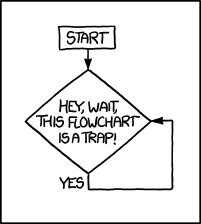
\includegraphics{illustration/tyomalli.png}
\caption{\label{tyomalli} Kuva työmallista}
\end{figure}

\hypertarget{tyuxf6mallin-haasteita}{%
\section{Työmallin haasteita}\label{tyuxf6mallin-haasteita}}

Tämä työmalli vaatii ohjelmoijalta paljon. Se edellyttää jatkuvaa
kiinnostusta sovellusalueen piirteistä, ja laajaa tarkkaavuutta
suunnittelutapaamisten keskuisteluissa. Lisäksi se edellyttää kykyä
sietää epävarmuutta ja muuttaa suunnitelmia usein ja isosti. Teknisellä
tasolla työmalli edellyttää kykyä joustavan ohjelmiston
suunnittelemiseen, laajojen refaktorointien tekemiseen kireässä
aikataulussa pysyen ja tiukkaa keskittymistä niihin päämääriin, jotka
mallin kehittämisessä on kulloinkin asetettu.

Jotta tällainen työmalli voi olla hedelmällinen tuotantotasoisen
ohjelmiston tekemisessä, se edellyttää myös, että työtyyli ohjelmoijan
ympärillä vastaa tällaista tekemisen tapaa. Liiketoimintavetoisella
suunnittelulla on vaikutuksia paitsi ohjelmistotuotannon prosessiin,
myös sitä ympäröiviin prosesseihin, kuten asiakastarpeiden kokoamiseen
ja tulevan kehitystyön suunnittelemiseen.
